\documentclass[11pt]{article}
\usepackage{amsmath,amsfonts,latexsym,graphicx}
\usepackage{fullpage}
\usepackage{url,hyperref}
\usepackage{subfig}
%\usepackage{ijcai09}

\pagestyle{empty}

\setlength{\oddsidemargin}{0in}
\setlength{\topmargin}{0in}
\setlength{\textwidth}{6.5in}
\setlength{\textheight}{8.5in}

\newtheorem{fact}{Fact}[section]
\newtheorem{lemma}{Lemma}[section]
\newtheorem{theorem}[lemma]{Theorem}
\newtheorem{assumption}[lemma]{Assumption}
\newtheorem{definition}[lemma]{Definition}
\newtheorem{corollary}[lemma]{Corollary}
\newtheorem{prop}[lemma]{Proposition}
\newtheorem{claim}[lemma]{Claim}
\newtheorem{remark}[lemma]{Remark}
\newtheorem{prob}{Problem}
\newtheorem{conjecture}{Conjecture}


\newenvironment{proof}{\vspace{-0.15in}\noindent{\bf Proof:}}%
        {\hspace*{\fill}$\Box$\par}
\newenvironment{proofsketch}{\noindent{\bf Proof Sketch.}}%
        {\hspace*{\fill}$\Box$\par\vspace{4mm}}
\newenvironment{proofof}[1]{\smallskip\noindent{\bf Proof of #1.}}%
        {\hspace*{\fill}$\Box$\par}

\newcommand{\etal}{{\em et al.}\ }
\newcommand{\assign}{\leftarrow}
\newcommand{\eps}{\epsilon}

%\newtheorem{lemma}{Lemma}
%\newtheorem{theorem}[lemma]{Theorem}
\begin{document}

\title{Information Set Generation in Kriegspiel}
\author{Abhishek Gupta	Mark Richards	Osman Sarood\\University of Illinois at Urbana-Champaign\\CS598LVK: Parallel Combinatorial Search\\Fall 2010}
\maketitle

\begin{abstract}
Information Set Generation is the identification of the set of paths in an imperfect information game tree that are consistent with a player's observations.  The ability to reason about the possible state of the world is crucial to the performance of game playing agent's.  In this work, we discuss the problem of information set generation in the context of kriegspiel (partially observable chess).  We implement the algorithm on top of a general purpose combinatorial search engine and discuss its performance under different load balancing strategies.  We discuss some variations in the search strategy and their effect on performance.
\end{abstract}

\section{Introduction}
In imperfect inormation games, players do not have access to full knowledge of the world. Examples of imperfect information include hidden cards in Poker or Bridge, hidden tiles in Scrabble, or hidden pieces in Stratego or Kriegspiel (partially observable chess). The game tree nodes that are indistinguishable to a player because they differ only in the information that is hidden to the player by rule are called that player's information set. The ability to estimate the value of the possible states and to reason about the probability distribution over those states is crucial to playing imperfect information games well. While it is often not possible to consider all nodes in an information set, it can be helpful to sample from them. Solving the problem would have the flavor of an all-solutions search. Good results on Kriegspiel specifically or an approach that works well on a variety of games should be publishable.

For many games, solving the information set generation problem is trivial.  For example, in a poker game, it is easy to see that the unseen cards held by a player's opponents may be any permutation of the cards not seen by that player (i.e., hole cards and any revealed community cards).  After the betting rounds, it would not be reasonable to assume that each of these permutations of unseen cards is equally probable, as betting decisions made by the players up to that point would be affected by the quality of those players' cards.  But the set of {\em possible} hands for all of the opponents is easy to conceive and enumerate.

In the game of kriegspiel, information set generation is non-trivial.  The player knows the opponent's position with certainty when the game begins, but after the initial move there may be varying levels of uncertainty about the location of the opponent's pieces.  Unlike poker, it is not possible to simply permute all of the opponent's possible pieces over all of the squares not occupied by the player's own pieces.  A configuration of pieces for the opponent is only valid.
Information set generation is not the same problem as solving a game tree, although it is arguably a necessary subroutine for quality game play in imperfect information games. The standard game tree problem is to find an equilibrium (i.e., minimax) strategy for the game. This can be done using alpha-beta pruning for perfect information games or linear programming for imperfect information games. Information set generation, by contrast, is the problem of finding sequences of moves in the game tree that are consistent with a player's observations.

And now I make a reference to Figure~\ref{fig:init}.
\begin{figure}
\begin{minipage}{\textwidth}
\centering
\subfloat[1. d4]{\label{fig:1W}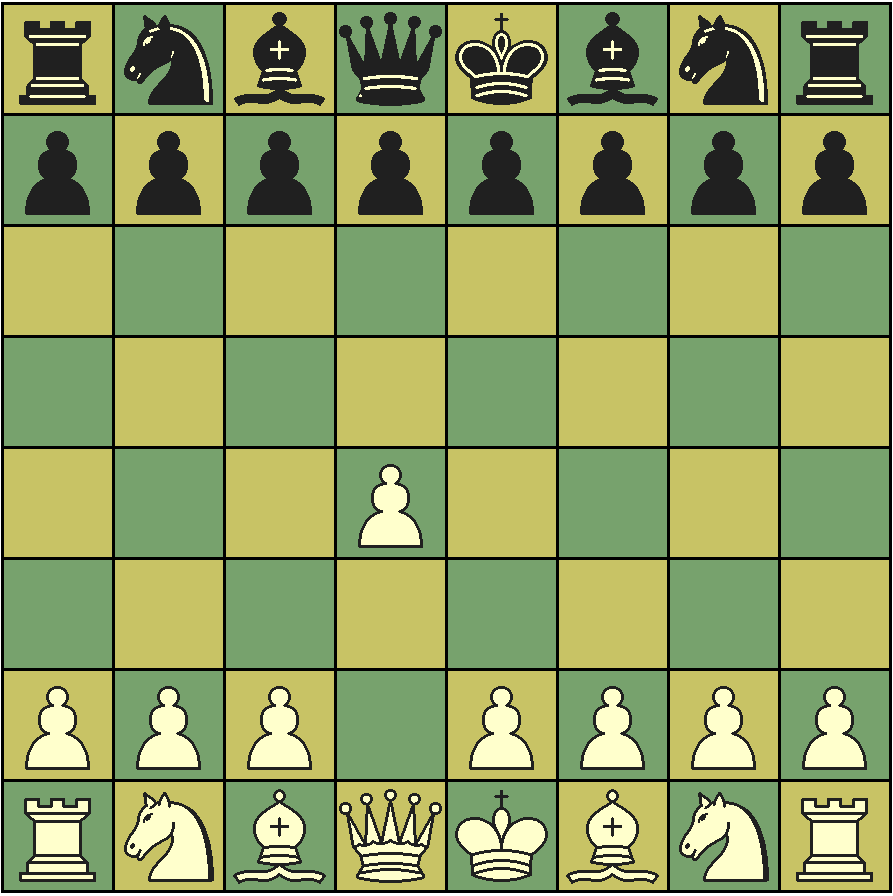
\includegraphics[width=0.2\textwidth]{images/1W.png}}
\qquad
\subfloat[1. ... a5]{\label{fig:1B}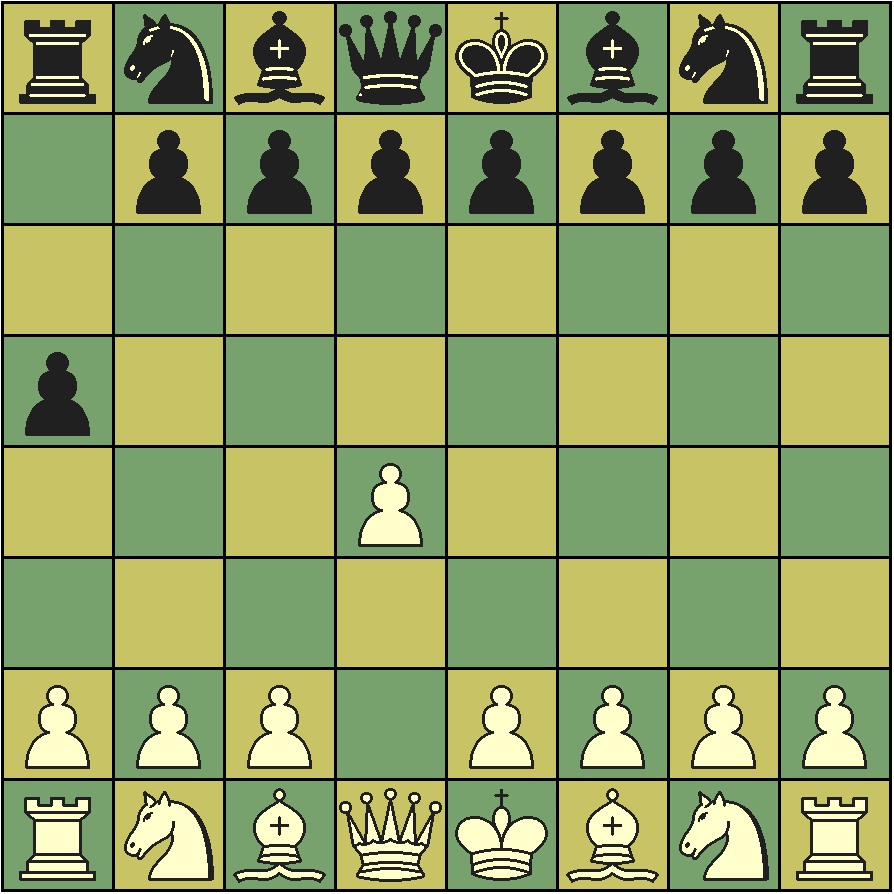
\includegraphics[width=0.2\textwidth]{images/1B.png}}
\qquad
\subfloat[2. Bg5]{\label{fig:2W}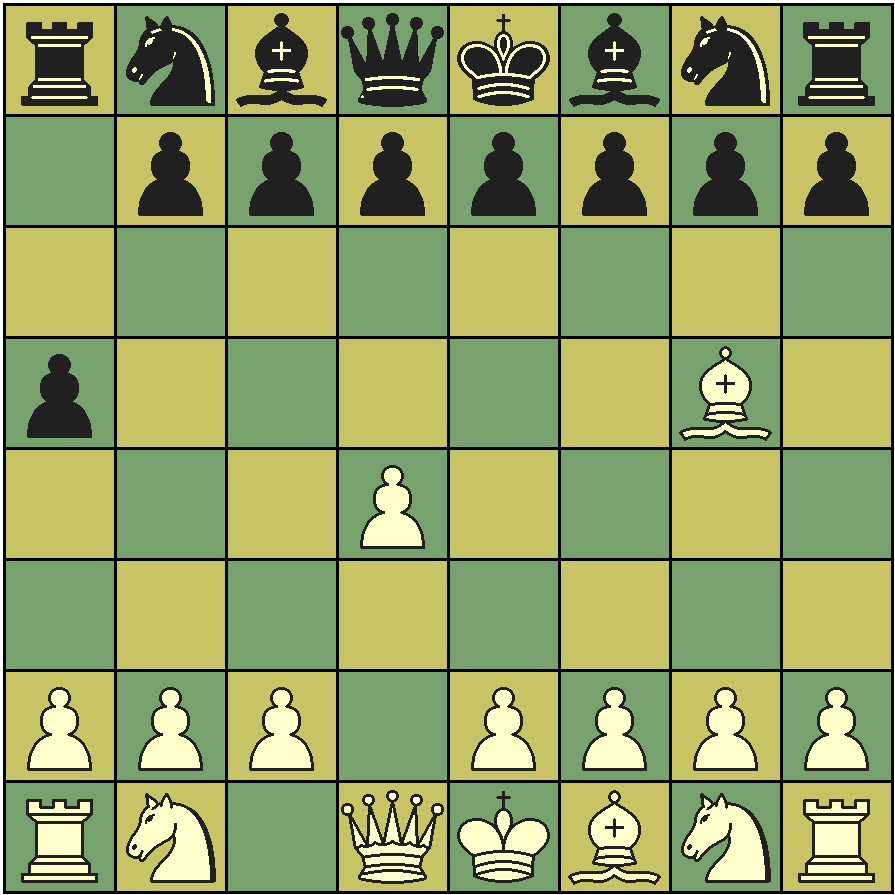
\includegraphics[width=0.2\textwidth]{images/2W.png}}
\qquad
\subfloat[2. ... b6]{\label{fig:2B}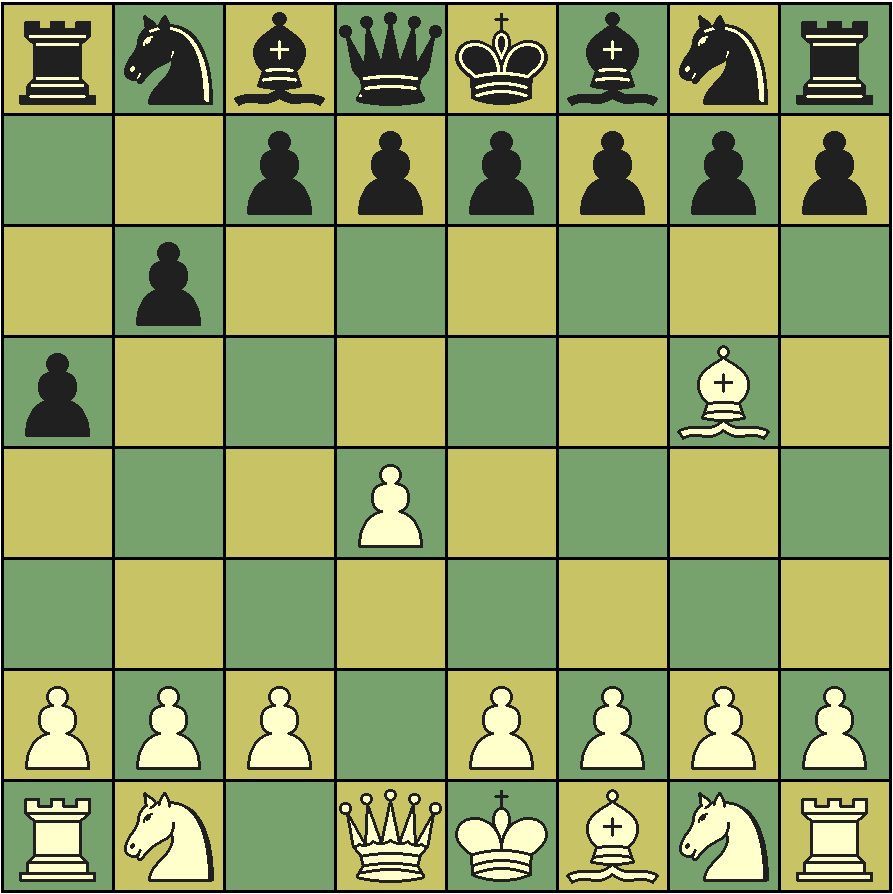
\includegraphics[width=0.2\textwidth]{images/2B.png}}
\end{minipage}
\begin{minipage}{\textwidth}
\centering
\subfloat[3. Nc3]{\label{fig:3W}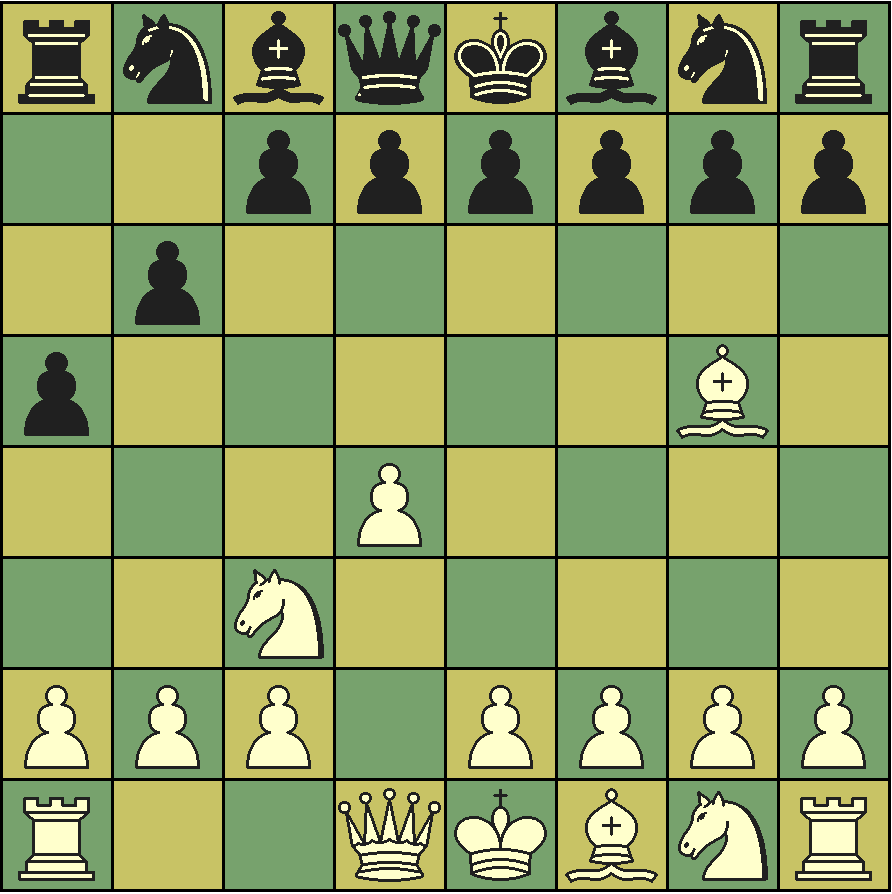
\includegraphics[width=0.2\textwidth]{images/3W.png}}
\qquad
\subfloat[3. ... c5]{\label{fig:3B}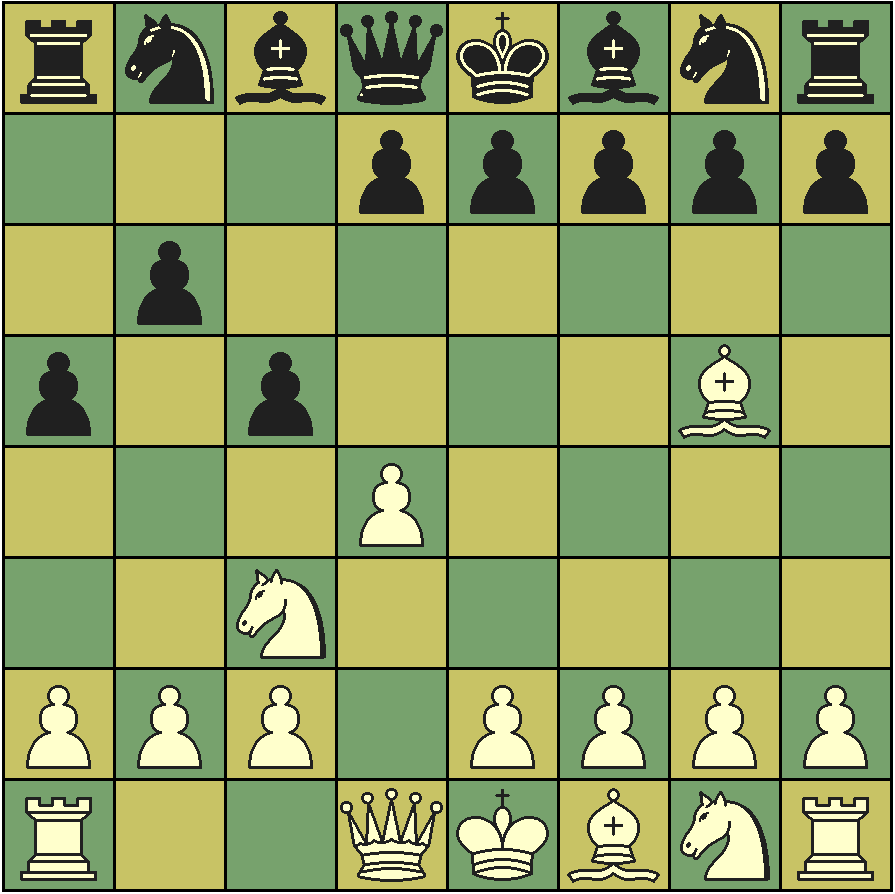
\includegraphics[width=0.2\textwidth]{images/3B.png}}
\qquad
\subfloat[4. d5]{\label{fig:4W}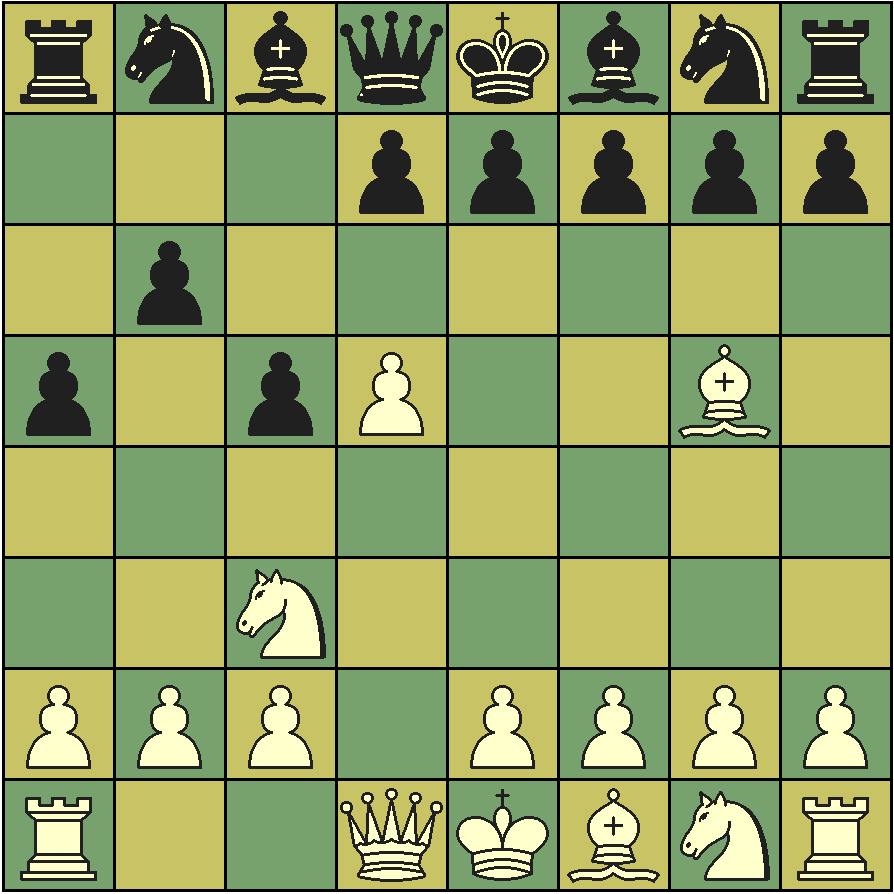
\includegraphics[width=0.2\textwidth]{images/4W.png}}
\qquad
\subfloat[4. ... Na6]{\label{fig:4B}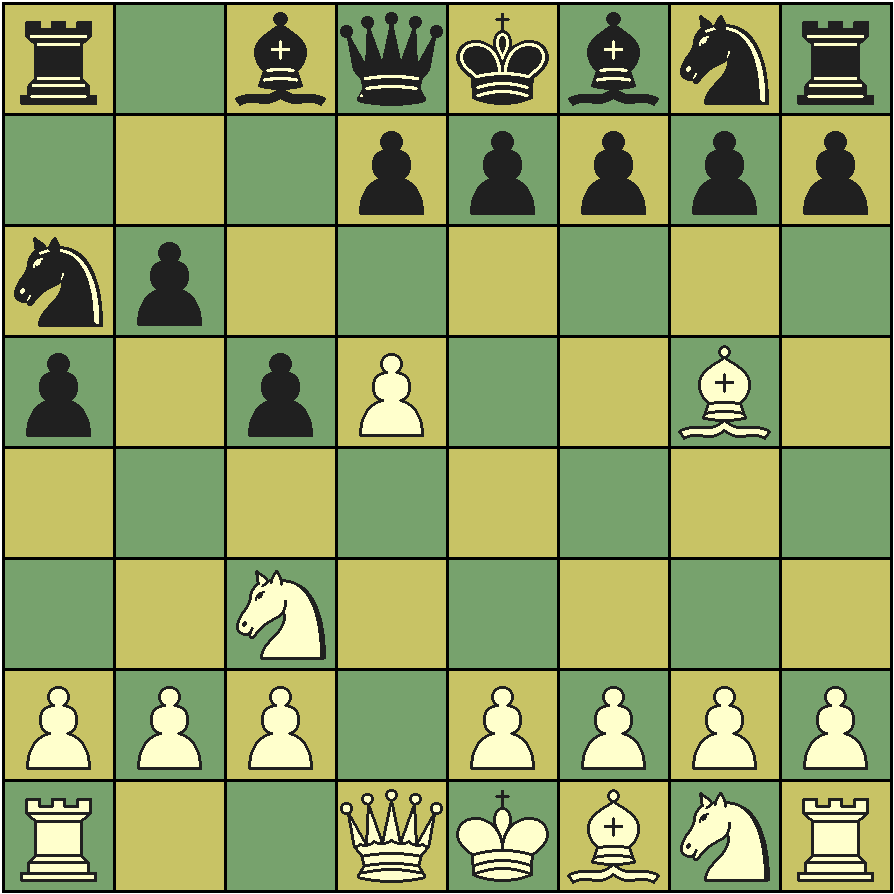
\includegraphics[width=0.2\textwidth]{images/4B.png}}
\end{minipage}
\begin{minipage}{\textwidth}
\centering
\subfloat[5. d6!]{\label{fig:5W}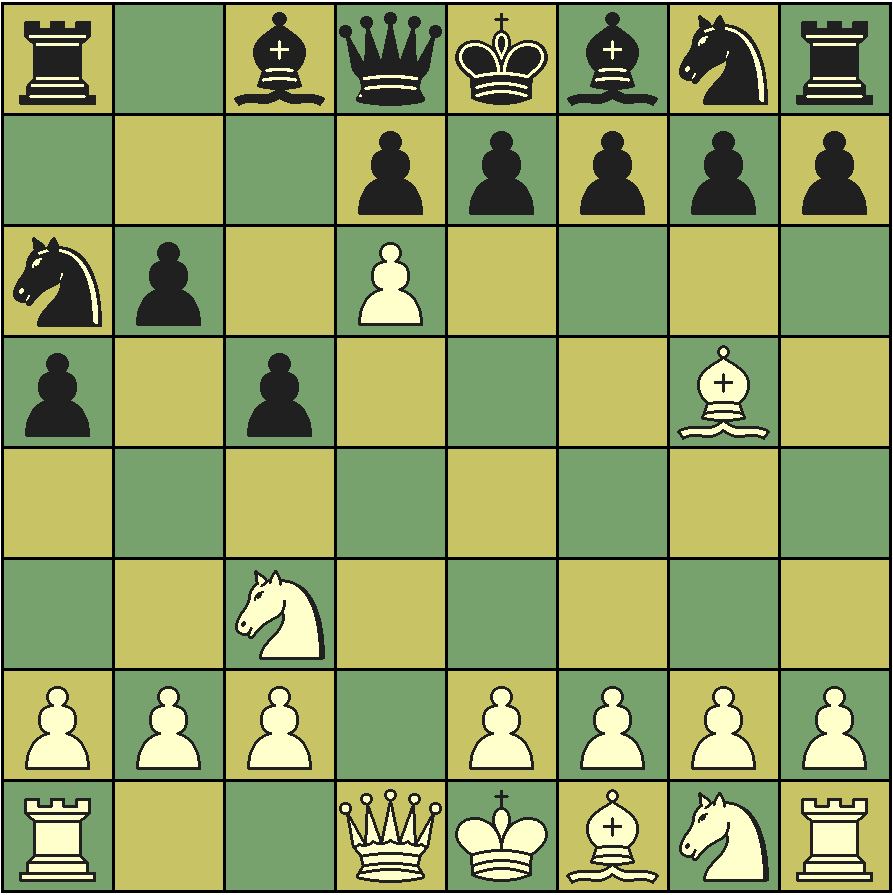
\includegraphics[width=0.2\textwidth]{images/5W.png}}
\qquad
\subfloat[5. ... f6!]{\label{fig:5B}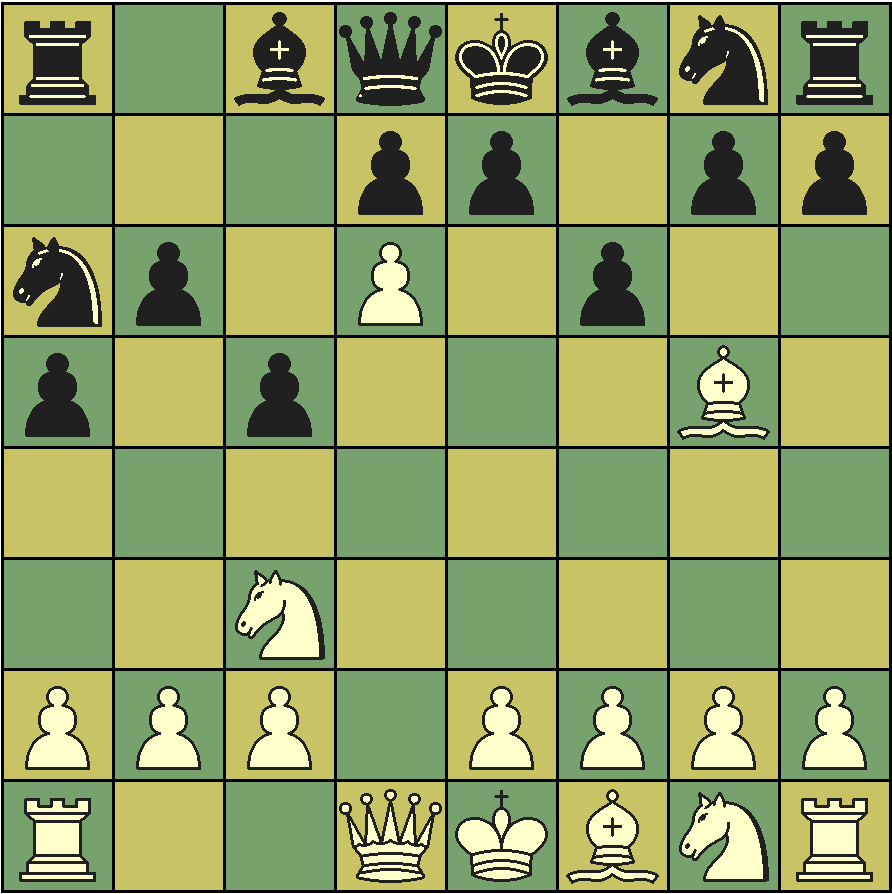
\includegraphics[width=0.2\textwidth]{images/5B.png}}
\qquad
\subfloat[6. e4]{\label{fig:6W}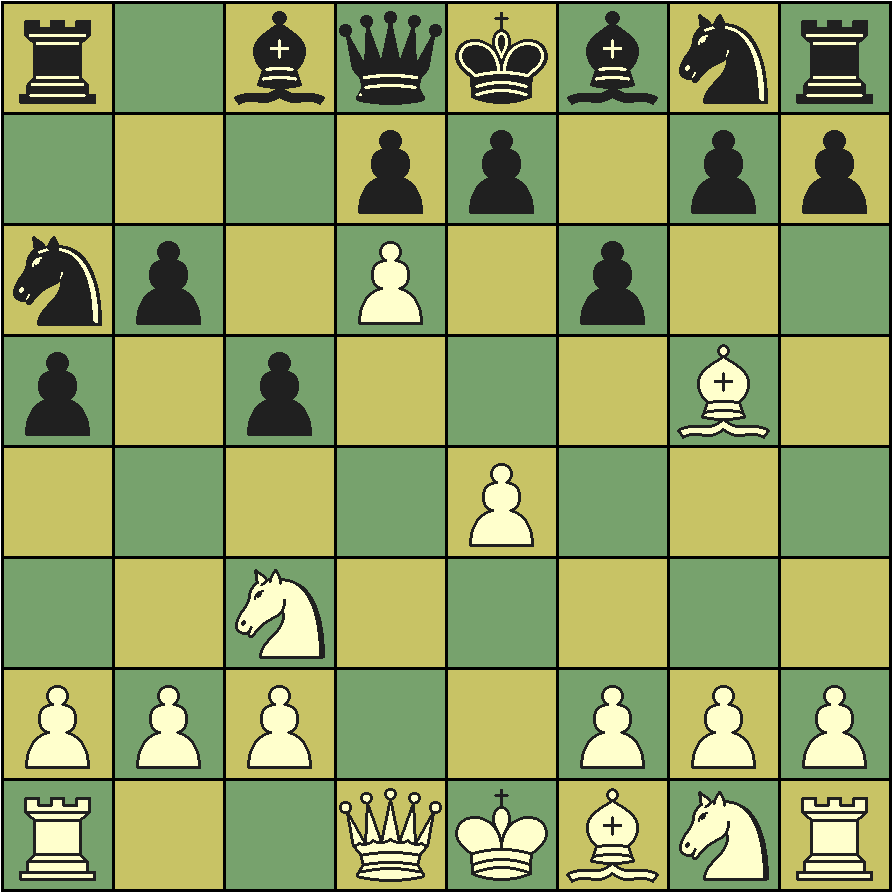
\includegraphics[width=0.2\textwidth]{images/6W.png}}
\qquad
\subfloat[6. ... fg]{\label{fig:6B}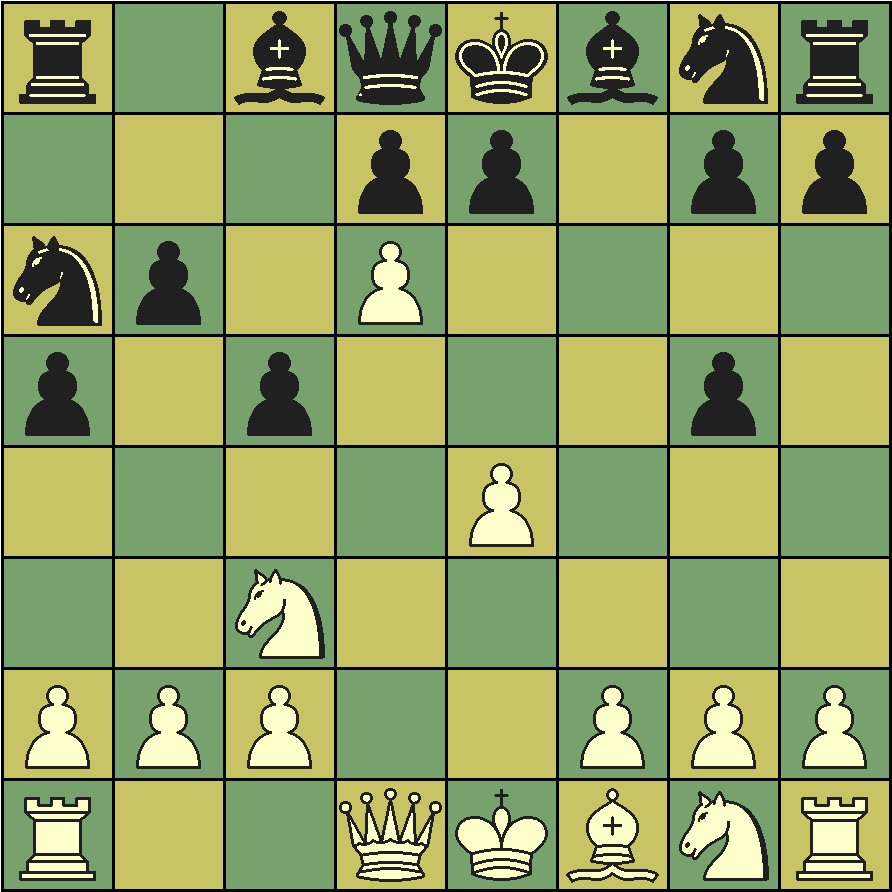
\includegraphics[width=0.2\textwidth]{images/6B.png}}
\end{minipage}
\begin{minipage}{\textwidth}
\centering
\subfloat[7. Bc4]{\label{fig:7W}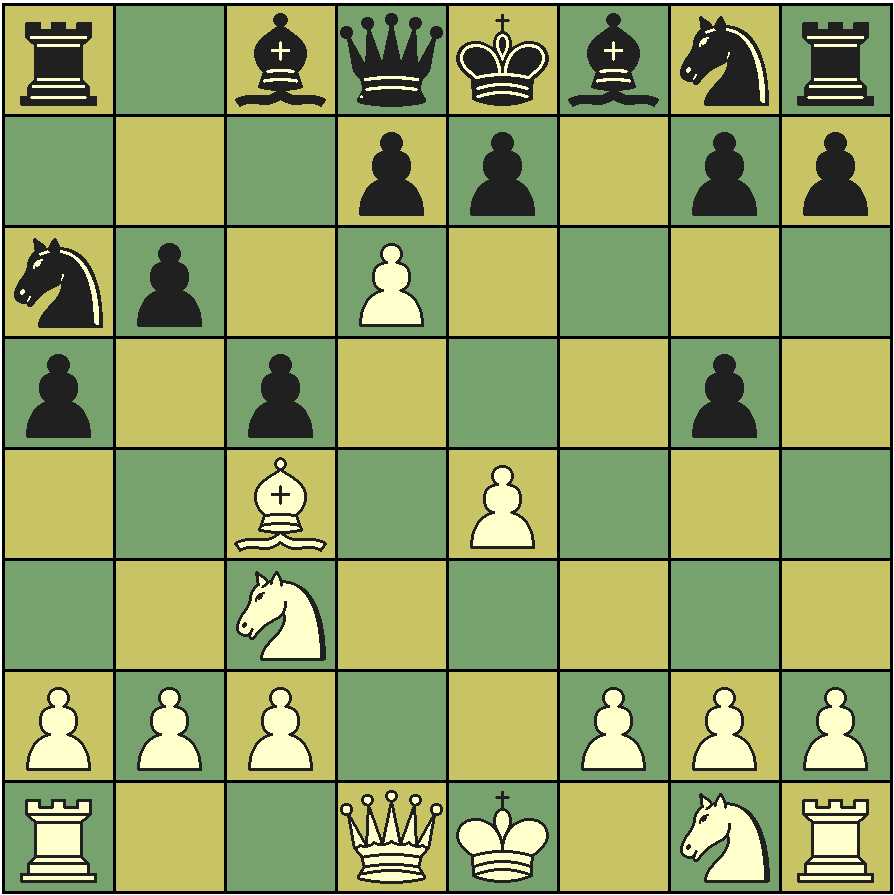
\includegraphics[width=0.2\textwidth]{images/7W.png}}
\qquad
\subfloat[7. ... ed]{\label{fig:7B}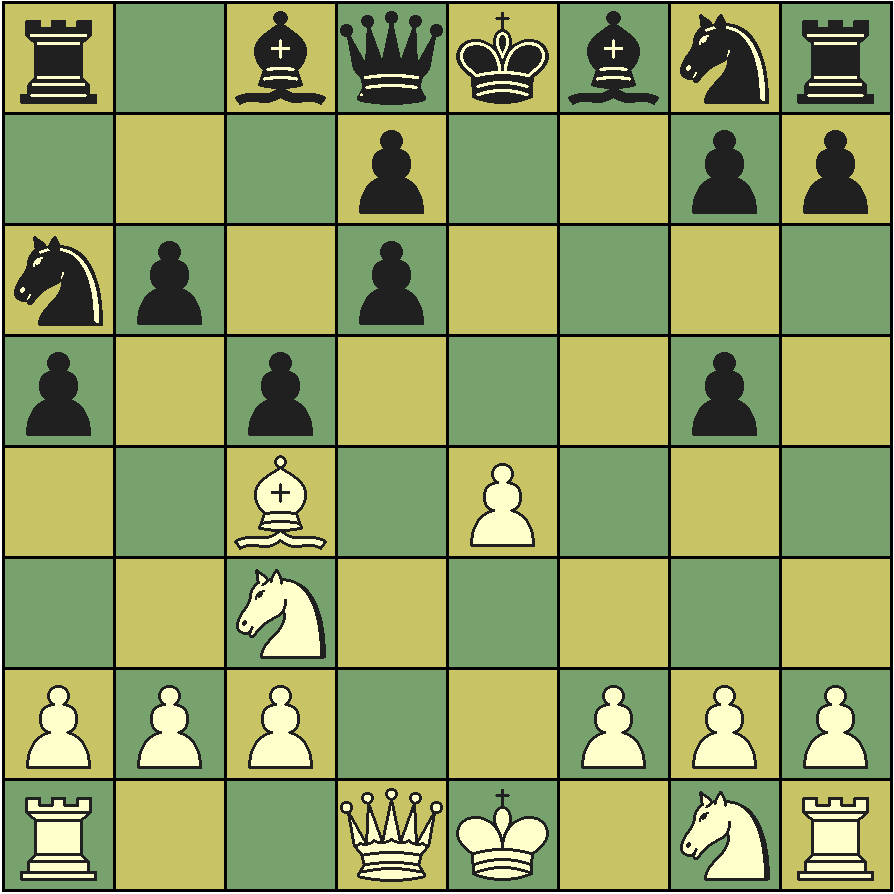
\includegraphics[width=0.2\textwidth]{images/7B.png}}
\qquad
\subfloat[8 Qd5!]{\label{fig:8W}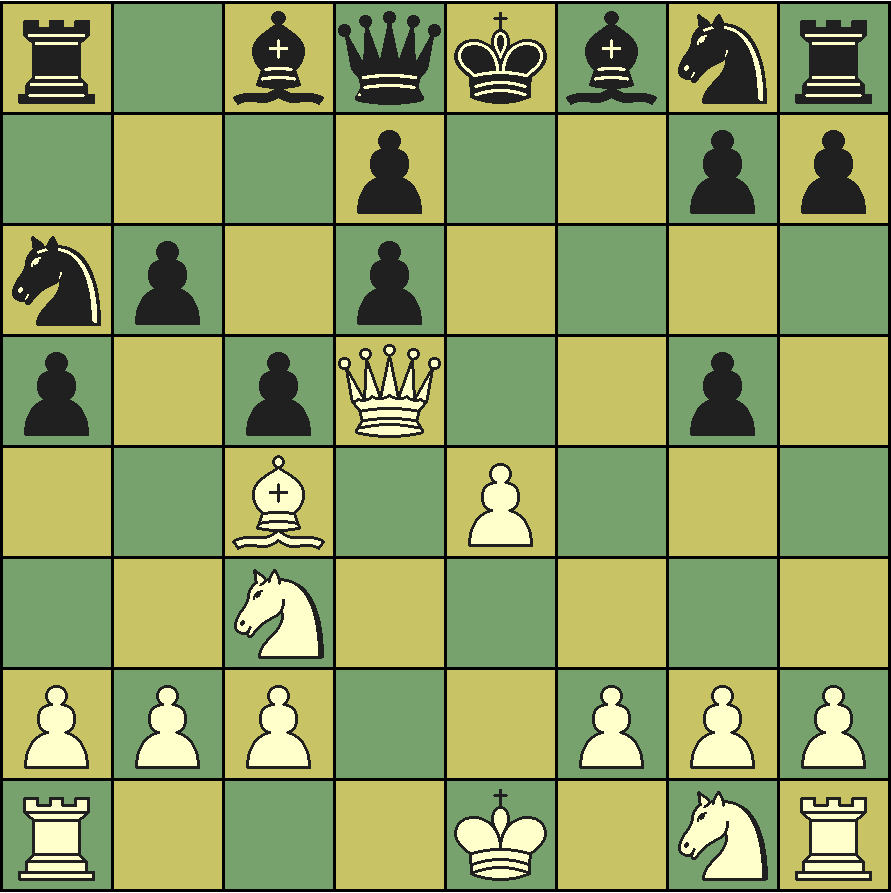
\includegraphics[width=0.2\textwidth]{images/8W.png}}
\qquad
\subfloat[8 ... Qc7?]{\label{fig:8B}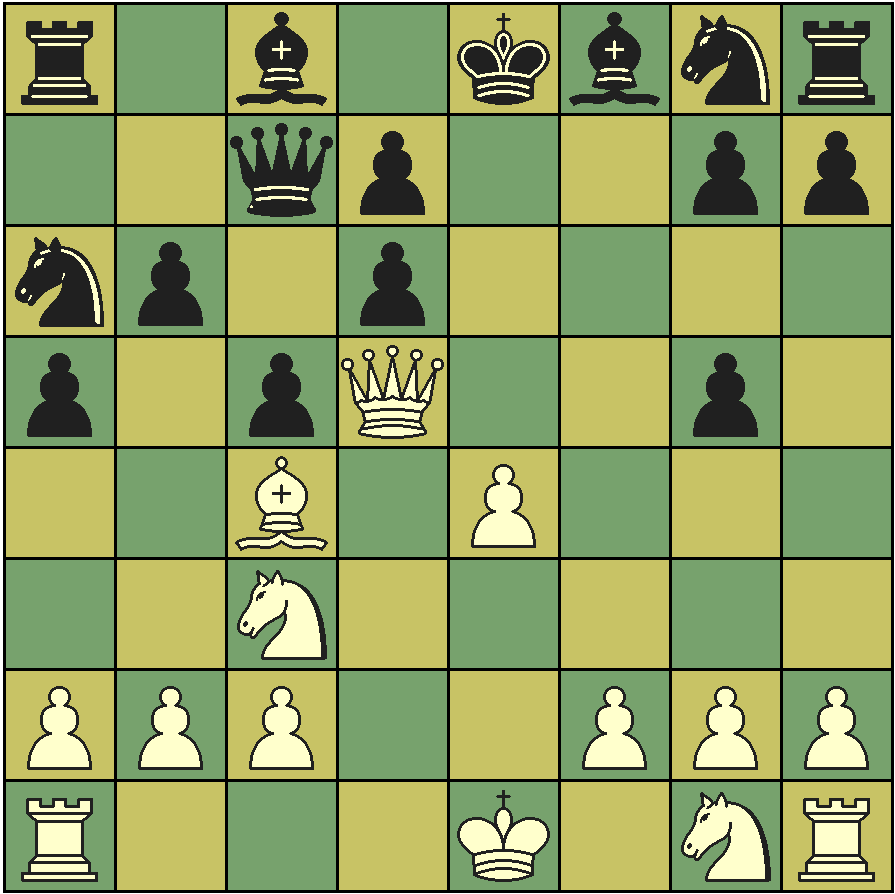
\includegraphics[width=0.2\textwidth]{images/8B.png}}
\end{minipage}
\begin{minipage}{\textwidth}
\centering
\subfloat[9 Qf7+]{\label{fig:9W}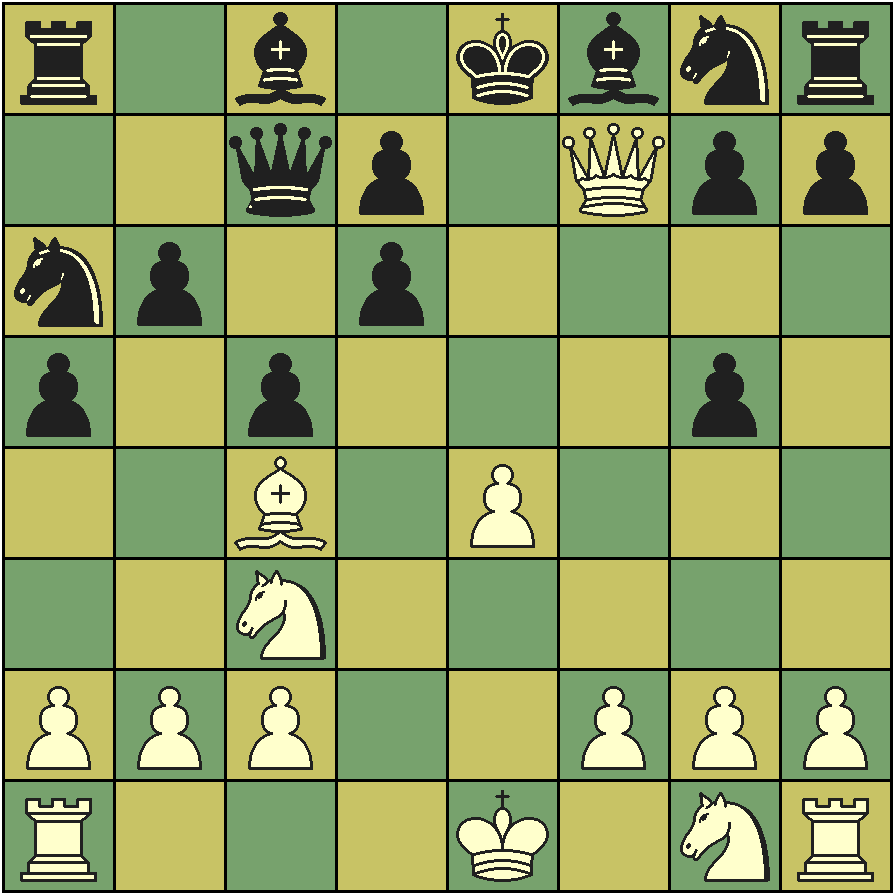
\includegraphics[width=0.2\textwidth]{images/9W.png}}
\qquad
\subfloat[9 ... d8]{\label{fig:9B}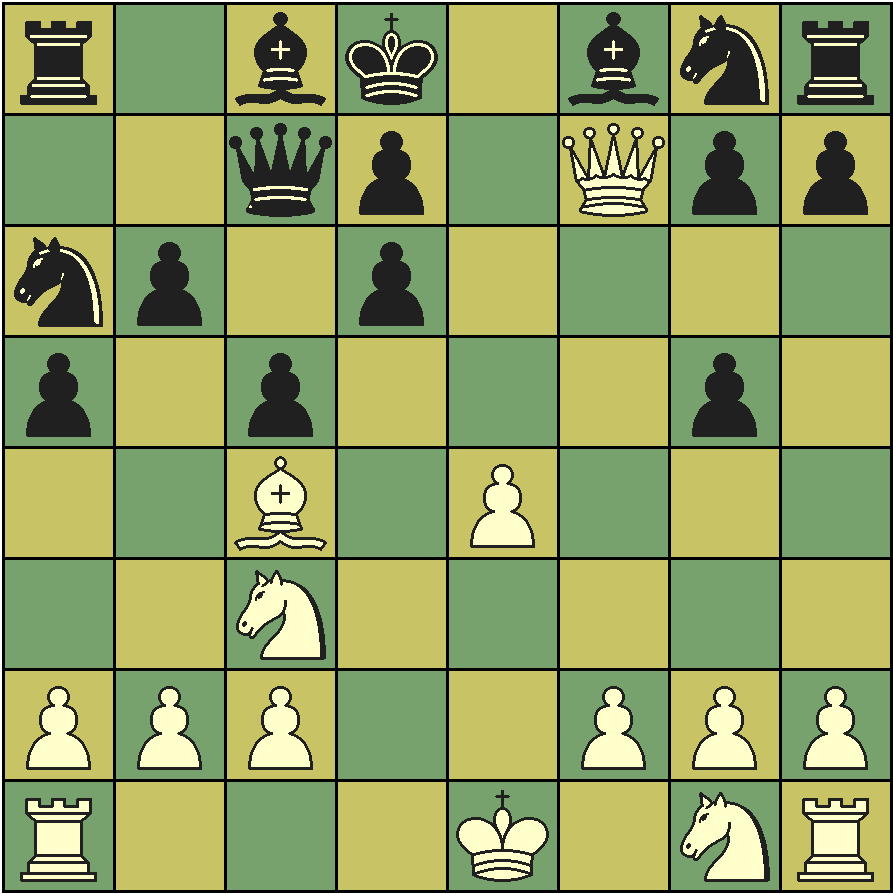
\includegraphics[width=0.2\textwidth]{images/9B.png}}
\qquad
\subfloat[10 Qxf8++]{\label{fig:10W}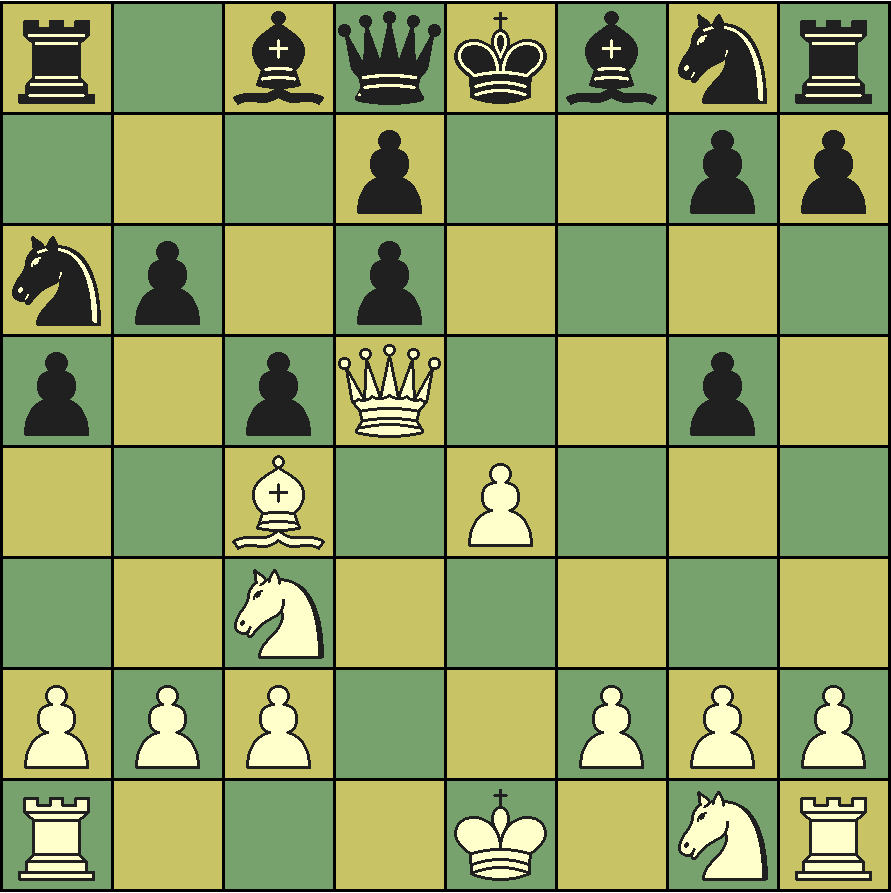
\includegraphics[width=0.2\textwidth]{images/8W.png}}
\end{minipage}
\caption{Sequence of moves}
\label{fig:sequence}
\end{figure}
%\nocite{*}
\nocite{richards09information}
\nocite{russell05efficient}
\nocite{kuhn03lectures}
\nocite{kuhn97classics}
\nocite{parker05sampling}
\nocite{nance06reasoning}
\nocite{li94chess}

\bibliographystyle{acm}
\bibliography{paper}
%\begin{thebibliography}{99}
%\end{thebibliography}

\end{document}
